\framework takes a sequence of Arabic words 
$T=\langle t_1,t_2,\ldots,t_M\rangle$ as input text, 
a set of tag types ${\cal T}$ each with its Boolean or sequential formulae. 
\framework is integrated with {\em Sarf}, 
an open source Arabic morphological analyzer based on finite state transducers~\cite{ZaMaColing2012DemosSarf}. 
\framework uses Sarf to compute a set of morphological solutions $M(t_i)=\{m_1,m_2,\ldots,m_N\}$
for each word $t_i, 1\le i \le M$.

\def\pp{\ensuremath{{\cal P}}} % prefix
\def\ss{\ensuremath{{\cal S}}} % stem
\def\xx{\ensuremath{{\cal X}}} % suffix
\def\PP{\ensuremath{\mathit{POS}}} % pos
\def\GG{\ensuremath{\mathit{GLOSS}}} % gloss
\def\AC{\ensuremath{\mathit{CAT}}} % category


Let \pp, \ss, \xx, \PP, \GG, and \AC~be the set of 
prefixes, stems, suffixes, POS tags, gloss tags, and abstract category tags
in our system.
Each morphological solution $m$ is of the form $\langle p,s,x,P,G,C\rangle$ 
where $p\in \pp, s\in \ss, x\in \xx, P \in \PP, G \in \GG,$ and $C \in \AC$. 

\subsection{$\{k\}Syn$}
Let E and A be the sets of all English and Arabic words respectively. 
Let G $\subset$ E be the set of English glosses. 
Let L $\subset$ A be the set of Arabic words in a given lexicon. 
Let S $\subset$ L be the set of stems in the given Arabic lexicon.
We define the following functions.\\
Let function $\alpha$: S $\rightarrow$ $2^G$, map input Arabic Lexicon stems to subsets of related English glosses; e.g. g$_{s} = \alpha(s)\subset$2$^{G}$.\\
Let function $\gamma$: L $\rightarrow$ $2^S$, map input Arabic Lexicon words to subsets of relevant Arabic stems; e.g. s$_{l} = \gamma(l)\subset$2$^{S}$.

Given an Arabic word w$\in$L, we define Syn(w) to be the set of Arabic words directly related to w under gloss map.\\
$Sy(w)=\{u\mid u\in S\land\exists s\in \gamma(w)\land~\alpha(u)\cap\alpha(s)\neq\phi\}$

We define Sy$^{i}$(w) to denote stems related to w using gloss map of order i recursively.\\
$Sy^{1}(w) = Sy(w)$.\\
$Sy^{i+1}(w)=\{u\mid u\in S\land\exists s\in Sy^{i}(w)\land~\alpha(u)\cap\alpha(s)\neq\phi\}$.

We define $\{k\}Syn(w)$ to be the union of Sy$^{i}(w)$ for i=$1\dots k$.\\
Formally, $\{k\}Syn(w) = \bigcup\limits_{i=1}^{k} Sy^{i}(w)$.

\subsection{Morphology-based Atomic terms (MAT)}
Let ${\cal O} = \{ \mathit{isA}, \mathit{contains}\}$ be the set of atomic term 
predicates, and let ${\cal F} = \{ \pp, \ss, \xx, \PP, \GG, \AC\}$ be the 
set of morphological features. 

A MAT $a(w)$ in a Boolean tag type formula takes a word $w$ 
and a constant value of a morphological features $CF$ as input and is of the form. 
\[
  a(w) := \exists m \in M(w). m=\langle p,s,x,P,G,C\rangle. r \circ CF
\]

where $\circ \in {\cal O}$, 
$r \in \{p,s,x,P,G,C\}$, $\exists A \in{\cal F}.r\in A,CF \in A$.

Informally, a MAT indicates that a solution vector exists where 
a feature from the solution contains or exactly matches a constant value for the 
feature specified by the user. 

Another form of an MAT is based on the K-Synonym feature. 
It takes a word $w$, a constant stem value $CS$ and a constant integer $k$ and checks whether a stem of w belongs to $\{k\}Syn$(CS). Formally,
\[
  a(w) := \exists s\in \gamma(w).s\in \{k\}Syn(CS)
\]

where $k\in\{1,\dots,7\}$

\subsection{Morphology-based Boolean formula (MBF)}

The \framework Boolean formula is of the following form.
\begin{itemize}
  \item $a$ is an MBF where $a$ is an MAT.
  \item $\neg f$ is an MBF where $f$ is an MAT. This is interpreted
    as the negation (complement) of words matching $f$. 
  \item $f \vee g$ where $f$ and $g$ are MBF. This is interpreted as 
    the disjunction (union) of words matching $f$ with the words matching $g$. 
\end{itemize}

\subsection{Morphology-based regular expression (MRE)}
The \framework sequential formula is of the following form.
\begin{itemize}
\item $m$ is an MRE where $m$ is an MBF.
\item $fg$ is an MRE where $f$ and $g$ is an MRE. This is interpreted as
the sequence MRE $f$ followed by MRE $g$.
\item $f*$ is an MRE where $f$ is an MRE. 
This operation refers to the Kleene star interpreted as
zero or more occurrences of MRE $f$.
\item $f+$ is an MRE where $f$ is an MRE. 
This operation is interpreted as one or more occurrences of MRE $f$.
\item $f$\textasciicircum$x$ is an MRE where $f$ is an MRE and $x \in \mathbb{N^*}$. 
This is interpreted as zero or more occurrences of MRE $f$ up to $x$.
\item $f?$ is an MRE where $f$ is an MRE. 
This is interpreted as zero or one occurrence of MRE $f$.
\item $f\& g$ is an MRE where $f$ is an MRE and $g$ is an MRE. 
This is interpreted as the occurence of MRE $f$ and MRE $g$.
\item $f|g$ is an MRE where $f$ is an MRE and $g$ is an MRE. 
This is interpreted as the occurence of MRE $f$ or MRE $g$.
\end{itemize}

\subsection{Computational Actions}
The computational actions are C++ based with access to word features referring to 
an MBF match. 
The features include text, position in text, length of word (count of characters), 
and the equivalent integer number if applicable. 

Each MRE is associated with pre-match and on-match actions. 
Pre-match actions are executed before a match of the MRE and on-match actions 
are executed upon finding a match for the MRE. 
The regular expression is associated with global declarations and library includes.

\subsection{Tag type}
The set of tag types ${\cal T}$ contains tuples of the form $\langle l,f,d\rangle$ 
where $l$ is a text label with a descriptive name of the tag type, 
$f$ is a \framework MBF or MRE, and $d$ is a visualization legend. 
The visualization legend describes how the tags should be displayed to the user 
and contains information such as the foreground and background color, the
font size, weight, and style. 

\begin{figure*}[t]
  \centering
  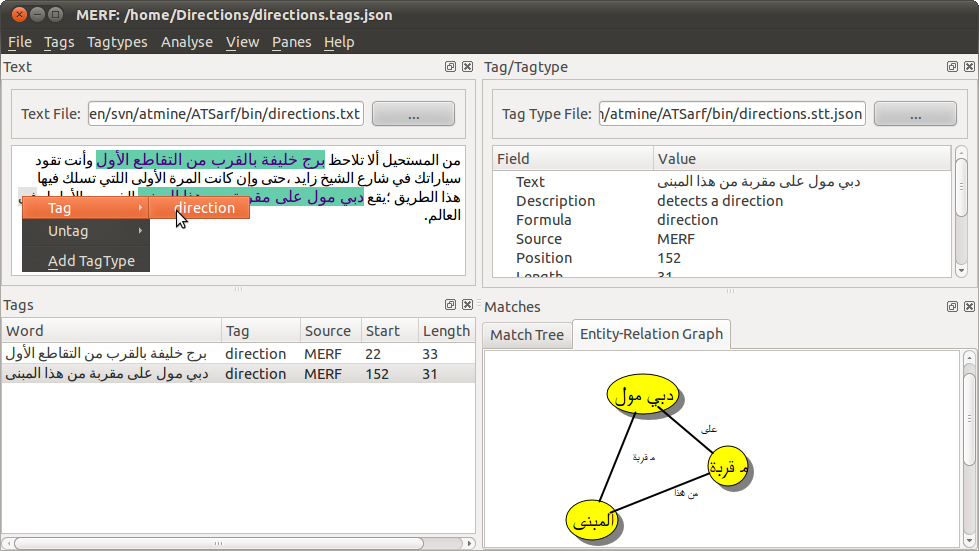
\includegraphics[width=0.9\textwidth]{figures/tagger}
  \caption{\framework main window with annotated text, tag descriptions, tag type legend properties, and manual tag edition menus. }
  \label{f:tagger}
\end{figure*}

\subsection{MBF Evaluation}
For each word $t_i \in T$, \framework computes a Boolean value 
($\{\mathit{true}, \mathit{false}\}$)
for all atomic terms. 
Then \framework computes Boolean values for all Boolean formulae. 
Then \framework computes the set of tags 
$R_i\subseteq T \times {\cal T}$  such that 
$(t_i,\mathit{tt}_j) \in R_i$ if and only if the Boolean formula $F_j$ associated with
tag type $\mathit{tt}_j$ is true for $t_i$. 

\subsection{MRE and Action Simulation}
For each MRE, 
\framework generates its equivalent non-deterministic finite automaton (NFA)~\cite{sipser2006introduction}. 
Each MRE operation has its equivalent representation in an NFA. 
As for the upto operation ($f$\textasciicircum$x$), 
it is equivalent to $f?|ff|\dots|\underbrace{f}_{n \text{ times}}$ which has an NFA mapping. 

Based on MBF evaluation stage, each word $t_i \in T$ is tagged by a tag set $R_i$. 
\framework simulates an NFA over the tag sets $R_i$ starting with $i=0,\dots,n$. 
A simulation match $m$ is a vector of the form $\langle r_i,r_{i+1},\dots,r_j\rangle$ where $0\le i\le j\le n~\text{and}~r_i\in R_i$. 
This tag match is equivalent to the text sequence match $\angle t_i,t_{i+1},\dots,t_j\rangle$ where $t_i\in T$. 

If the simulation has a match $\langle r_m,r_{m+1},\dots,r_n\rangle$ where $0\le m\le n\le n$, 
the next simulation starts at $R_{n+1}$. 
In case the NFA simulation has no match, the next simulation starts at $R_{m+1}$. 
If we have more than one match starting at $R_k$ where $0\le k\le n$, 
\framework returns the longest one.

\framework maintains a function $\phi\subset Q\times\Phi$, 
where $\mathit{Q}$ is the set of states in the NFA and $\Phi$ is the set of MREs in a formula. 
So $(q_i,f_j)\in\phi$ if state $q_i\in Q$ is generated by \framework in equivalence to $f_j\in\Phi$. 
\framework uses $\phi$ to retrieve the match tree with respect to the MRE formula. 
It also uses the map to execute the pre-match and on-match computational actions of an MRE based on current match.